%!TEX root = ../thesis.tex

\chapter{Розподіл секрету}
\label{chap:review1}  %% відмічайте кожен розділ певною міткою -- на неї наприкінці необхідно посилатись

\textbf{Розділення секрету} (англ. \textit{secret sharing}) \cite{keylessSS} --- це спосіб безпечного розповсюдження фрагментів важливої приватної інформації серед розподіленої мережі або групи, що робить такі схеми особливо корисними для захисту дуже чутливої інформації, наприклад, приватних криптографічних ключів або біометричних даних.

Розділення секрету працює шляхом поділу приватної інформації на менші частини -- або частки -- і подальшого розповсюдження цих часток серед групи або мережі.

Кожен окремий ресурс марний сам по собі, але коли всі ресурси зібрані разом, вони відновлюють початковий секрет.

\section{Існуючі схеми}
Існуючі схеми мають дві складові: розподіл і відновлення секрету. До поділу відноситься формування частин секрету і розподіл їх між членами групи, що дозволяє розділити відповідальність за секрет між її учасниками. Зворотна схема повинна забезпечити його відновлення за умови доступності його зберігачів у деякій необхідній кількості.

Схеми поділу секрету застосовуються у випадках, коли існує значна ймовірність компрометації одного або декількох зберігачів секрету, але ймовірність недобросовісної змови значної частини учасників вважається мізерно малою \cite{wikipedia}.

\vspace{0.25cm}
\textbf{Приклад розподілу секрету:} \par
Уявіть, що у вас є мільйон доларів, який ви зберігаєте на банківському рахунку, і для доступу до нього ви використовуєте пароль: secret. Ви могли б розділити його на частини і розіслати по одному листу шістьом довіреним акціонерам. Єдиною інформацією, яку матиме кожен акціонер, є лист, який він тримає на руках, що фактично робить його акції марними.

\begin{figure}[ht]
        \centering
        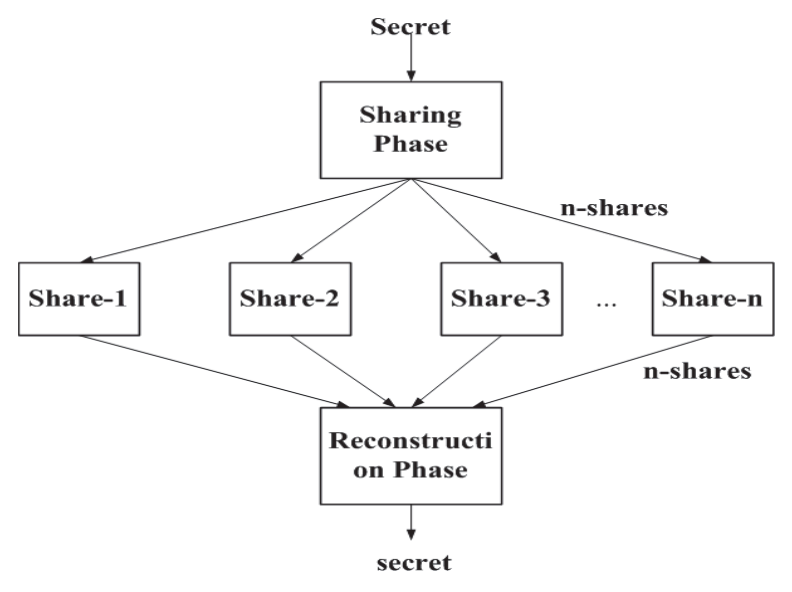
\includegraphics[scale=0.37]{IMAGES/SSscheme.png}
        \caption{Звичайна схема розподілу секрету}
        \label{fig_SSscheme}
\end{figure}
\vspace{-1cm}

\subsection{Ієрархічні схеми розподілу секрету}
Схеми розподілу секрету також можуть бути ієрархічними, залежно від того, як розподіляються частки секрету. Це дозволяє власнику секрету розподіляти частки залежно від того, наскільки акціонери йому довіряють.

\begin{figure}[ht]
        \centering
        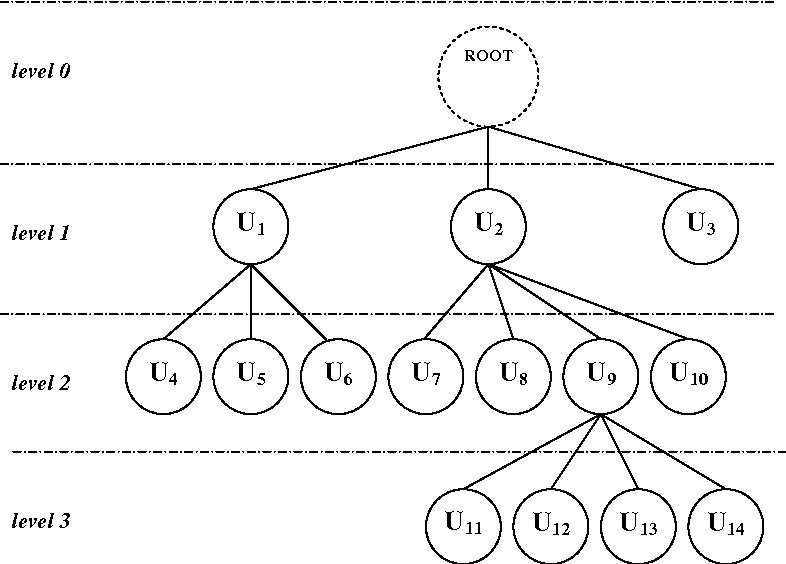
\includegraphics[scale=0.37]{IMAGES/hierarchical_SCscheme.png}
        \caption{Ієрархічна схема розподілу секрету}
        \label{fig_hierSSscheme}
\end{figure}

\textbf{Приклад ієрархічної схеми:} \par
Припустимо, ви хочете безпечно зберігати свій приватний ключ, який ви використовували для доступу до свого криптовалютного гаманця.
Закриті ключі використовуються для переказу криптовалюти з однієї адреси на іншу. Вони складаються з послідовності випадкових і унікальних чисел і надаються користувачам під час відкриття гаманця.

По-перше, ви не захочете давати комусь всю послідовність, тому, скажімо, розділите ключ на вісім частин. Потім ви розподіляєте копії цих частин між найближчими друзями та членами сім'ї, яким ви довіряєте.

Ви можете віддати по вісім частин кожному з батьків, яким ви беззаперечно довіряєте, по чотири частини брату і сестрі, яким ви довіряєте здебільшого, і по одній частині восьми друзям, яким ви довіряєте в деякій мірі. Така ієрархічна схема розподілу дозволяє власникам розподіляти частки секрету залежно від того, наскільки вони довіряють своїм акціонерам.

\subsection{Схеми розподілу секрету без довіри}
У більшості схем, в яких немає довіри між власником секрету та акціонерами, впроваджується додатковий рівень шифрування для забезпечення додаткової конфіденційності та безпеки. Це дозволяє розподіляти частки серед мережі або групи, які невідомі власнику секрету.

\vspace{0.25cm}
\textbf{Приклад схеми без довіри:}\par
Припустимо, що кожен акціонер володіє лише випадковими числами:~ 19, 5, 3, 18, 5, 20.

При шифруванні, коли всі окремі частки (числа) зібрані разом, вони все одно потребують ключа-дешифрувальника, щоб розкрити секрет (літери), які вони представляють в алфавіті.

Цей важливий крок захищає приватну інформацію від організованих атак; навіть якщо кожен акціонер вступить у змову, щоб відтворити оригінальний секрет, він не зможе нічого дізнатися про цей секрет, оскільки оригінальний секрет зашифрований.

\section{Проблема розподілу часток секрету}

Однією з проблем розподілу часток секрету є те, що вони часто можуть бути втрачені або скомпрометовані. Акціонери можуть померти, втратити свої частки або їх можуть вкрасти. А в разі втрати хоча б одного з членів групи, секрет буде загублений для всієї групи безповоротно. Інколи акціонери самі стають шахраями. Коли розподіляється багато різних часток, також непрактично і неефективно вимагати від усіх акціонерів відновити секрет.

\section{Порогова схема як вирішення проблеми}

Порогова схема (\textit{threshold scheme}) пропонує вирішення проблеми розподілу часток секрету.

\vspace{-0.5cm}
\begin{figure}[ht]
        \centering
        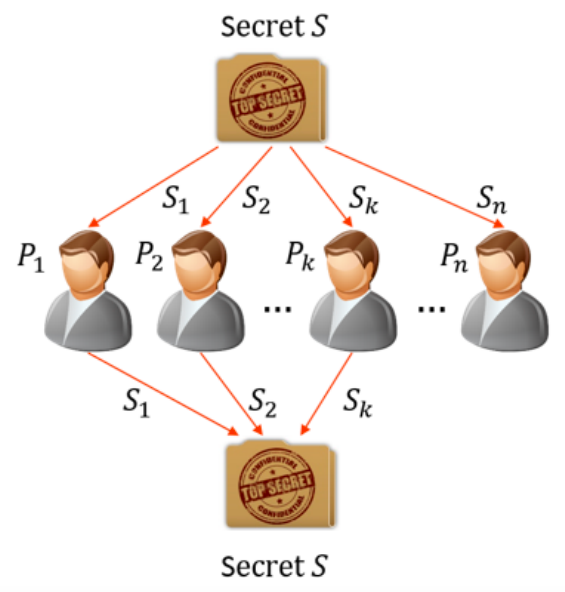
\includegraphics[scale=0.4]{IMAGES/thresholdSSS.png}
        \caption{Порогова схема розподілу секрету}
        \label{fig_thresholdSSscheme}
\end{figure}

\textbf{Порогова схема} --- це метод розподілу секрету, який дозволяє відновити секрет, навіть якщо деякі з часток секрету втрачені або скомпрометовані. Це відбувається завдяки тому, що для відновлення початкового секрету вимагається лише частина частинок секрету, на які був розділений.

\subsection{Найпростіша порогова схема}
Ви можете взяти будь-яке повідомлення (секретний рецепт, коди запуску, ваш список білизни тощо) і розділити його на n частин, які називаються тіньовими потоками або спільними ресурсами, так що будь-які m із них можна використовувати для реконструкції повідомлення. Це називається (m,n)-порогова схема.

\vspace{0.25cm}
\textbf{Приклад найпростішої порогової схеми:} \par
За допомогою (3,4)-порогової схеми Трент може розділити свій секретний рецепт соусу між Алісою, Бобом, Керол і Дейвом, щоб будь-які троє з них могли об’єднати свої тіні та реконструювати повідомлення. Якщо Керол у відпустці, Аліса, Боб і Дейв можуть це зробити. Якщо Боба переїде автобус, Аліса, Керол і Дейв зможуть це зробити. Однак, якщо Боба переїде автобус, коли Керол у відпустці, Аліса та Дейв не зможуть відновити повідомлення самостійно.

\subsection{Загальні порогові схеми}
Загальні порогові схеми ще більш універсальні. Будь-який сценарій спільного використання, який ви можете собі уявити, можна змоделювати. Ви можете розділити повідомлення між людьми у вашій будівлі так, щоб для його реконструкції вам знадобилося сім людей з першого поверху та п’ять людей з другого поверху якщо не буде залучено когось із третього поверху. У такому випадку вам лише потрібна ця особа та троє людей з першого поверху та двоє людей з другого поверху, за винятком випадків, коли хтось із четвертого поверху задіяний. У такому випадку вам потрібна ця особа та одна особа з третього поверху, або ця особа та двоє людей з перший поверх і одна особа з другого поверху і т.д.
Цю ідею винайшли незалежно один від одного Аді Шамір і  Джордж Блеклі, а також ретельно досліджував Гас Сіммонс в своїх алгоритмах.

\chapconclude{\ref{chap:review1}}

В цьому розділі ми розглянули важливу криптографічну задачу, яка дозволяє безпечно ділитися секретом між групою учасників -- розділення секрету. Також розглянули існуючі різні схеми розділення секрету, які мають різні характеристики та ступінь стійкості до атак; проблему розподілу часток секрету та її вирішення -- порогові схеми. В результаті було визначено, що розділення секрету є важливим інструментом для забезпечення безпеки та конфіденційності інформації. А порогові схеми -- це один із найефективніших способів розподілу секрету між групою учасників.